%!TEX program = xelatex

\documentclass[cn,black,9pt,normal]{elegantnote}
\usepackage{float}
\usepackage{hyperref}


%\newcommand{\upcite}[1]{\textsuperscript{\textsuperscript{\cite{#1}}}}

\title{数码摄影作业(07)人像\\\small{读书的人}}
\author{姓名:姜文渊\\学号:1951510}
%\institute{School of Life Science, Tongji University}
%\version{1.00}
\date{2021年4月25日}

\begin{document}

\maketitle


\section*{拍摄条件及使用器材简介}

作业中使用的相机为佳能 M200,使用的镜头均为为 TTArtisan 50mm f1.2,该镜头为定焦手动镜头,
价格低廉,但背景虚化较好,适合拍摄人像。

拍摄地点于我校三好坞后一园子中,感谢本班的同学\textbf{素颜}出镜。




\section{所摄照片}
\begin{figure}[H]
    \centering
    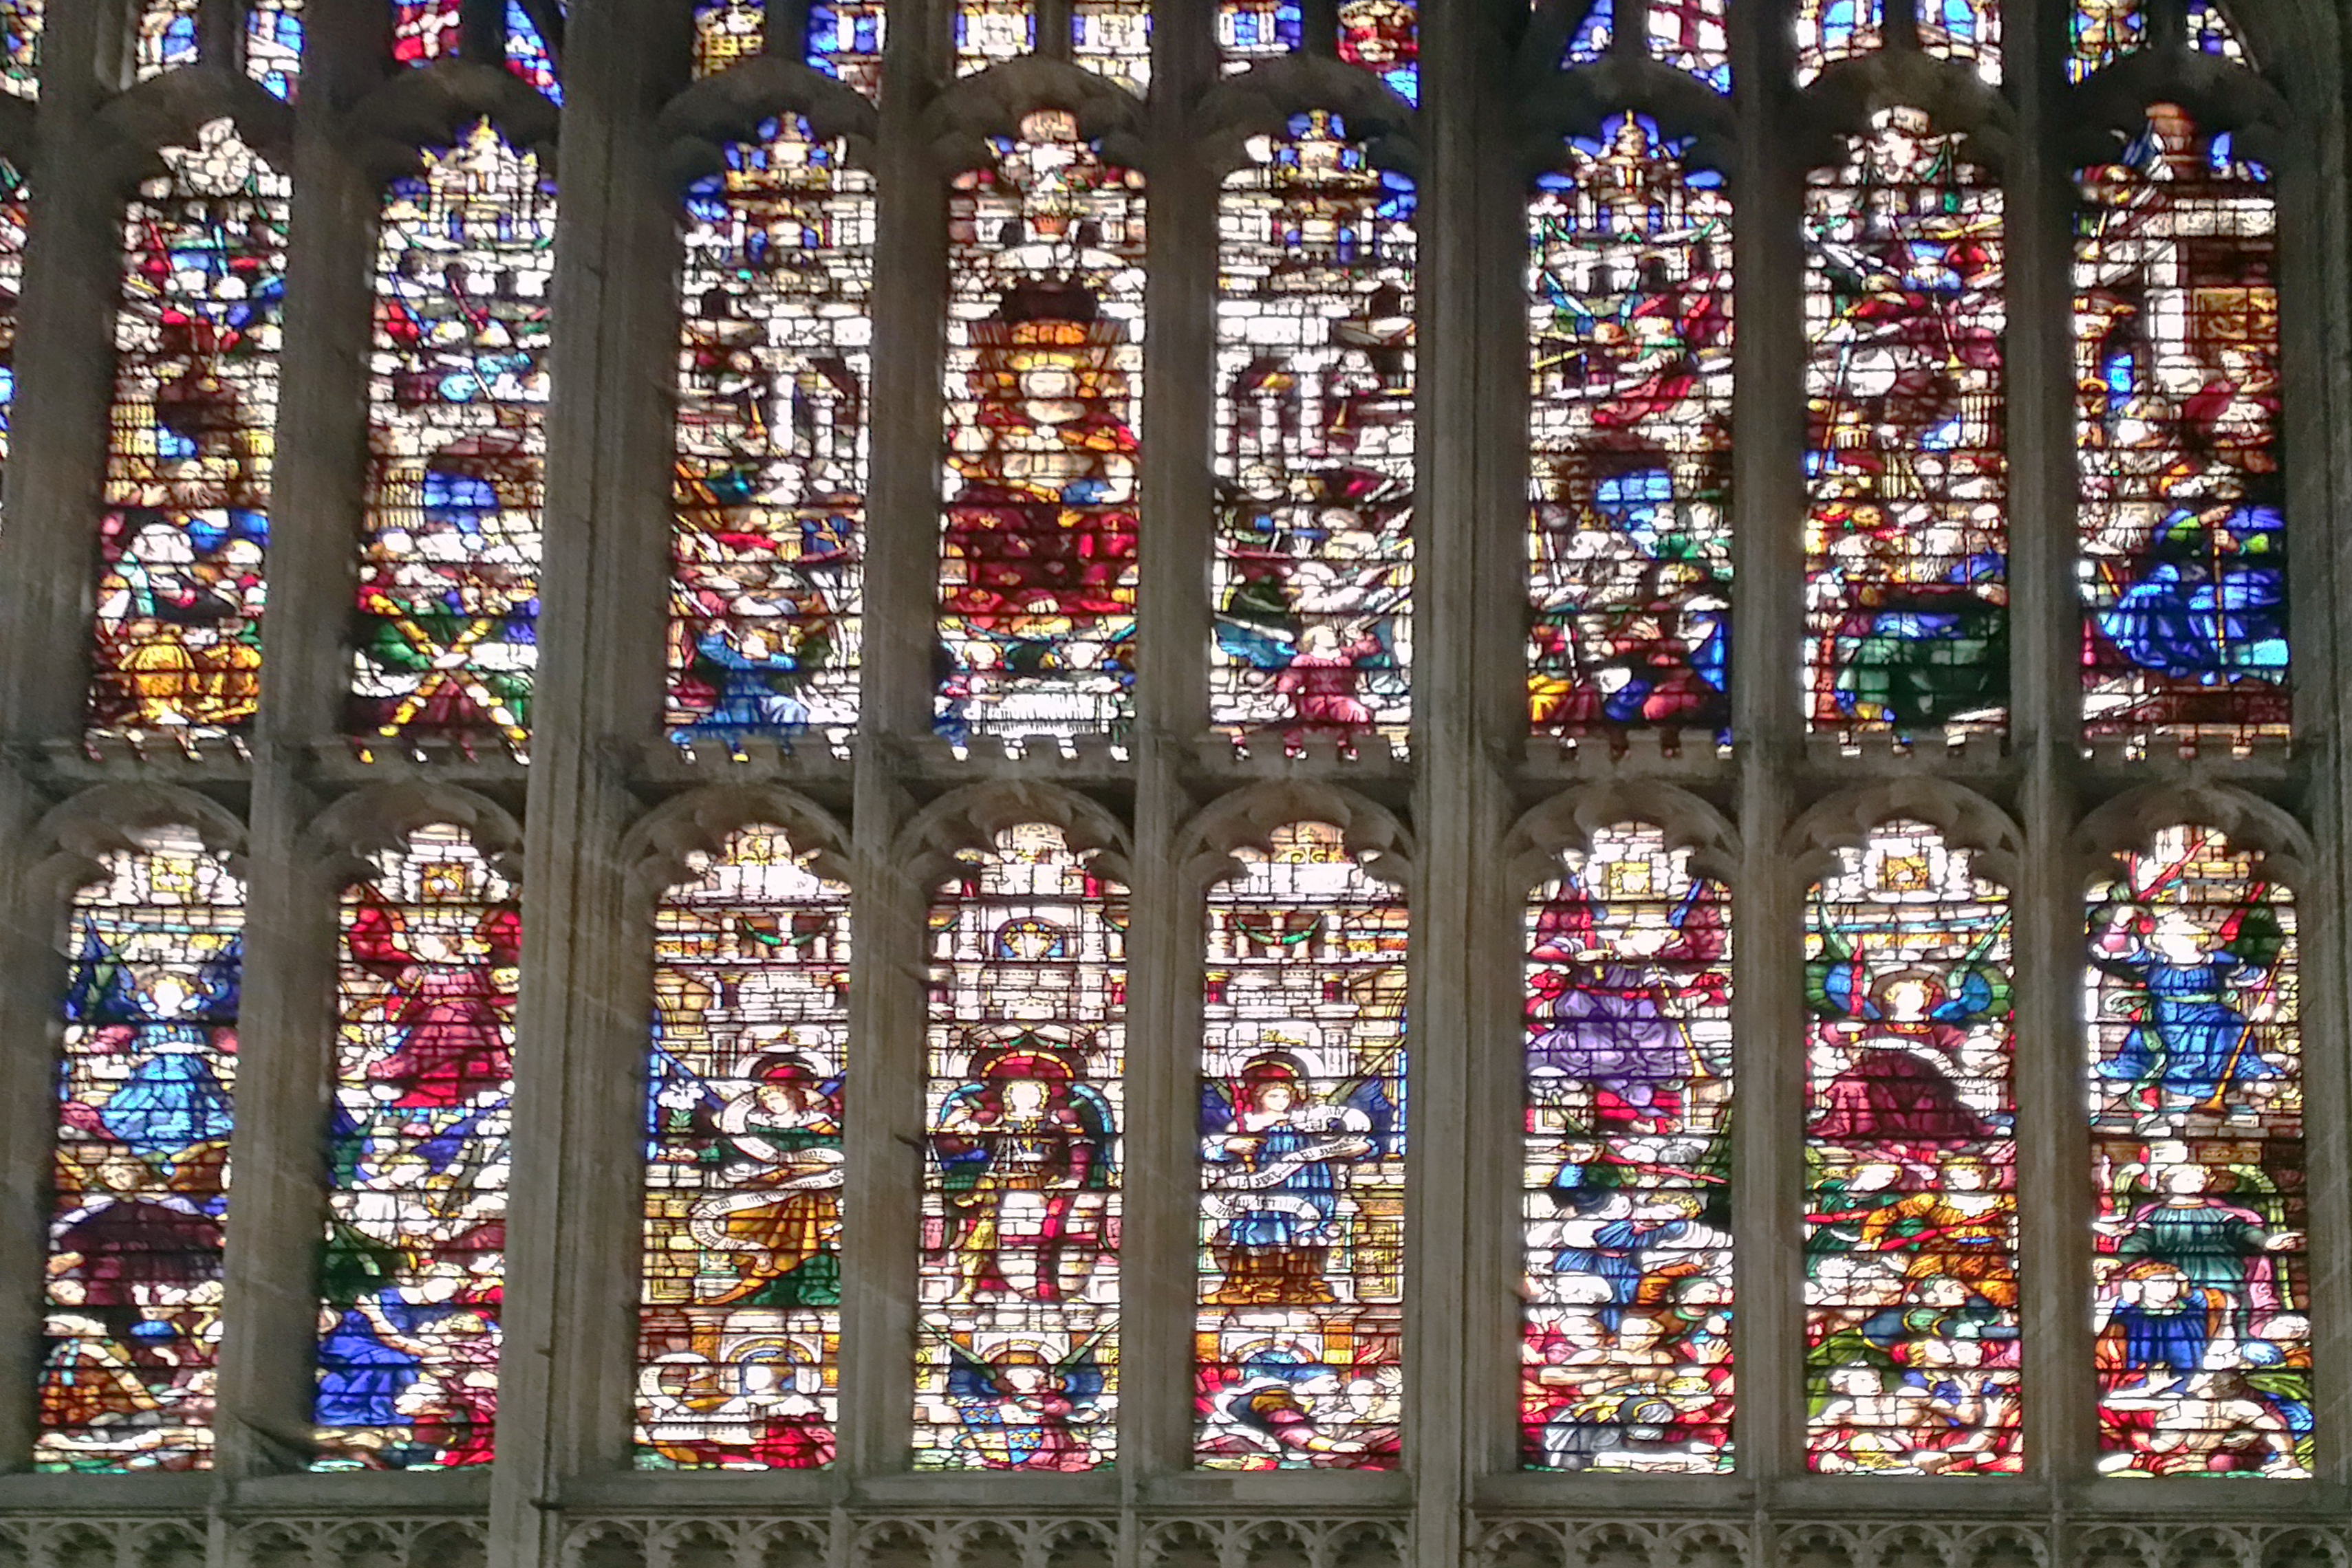
\includegraphics[width=0.8\textwidth]{F2}
    \caption{50mm f1.4 1/200}
    \label{F-02}
\end{figure}

上面的照片构图较为传统,主体位于画面中央。
被摄同学侧身而立,没有直接表现正脸,手持一本外文书籍。




\section{所摄照片}
\begin{figure}[H]
    \centering
    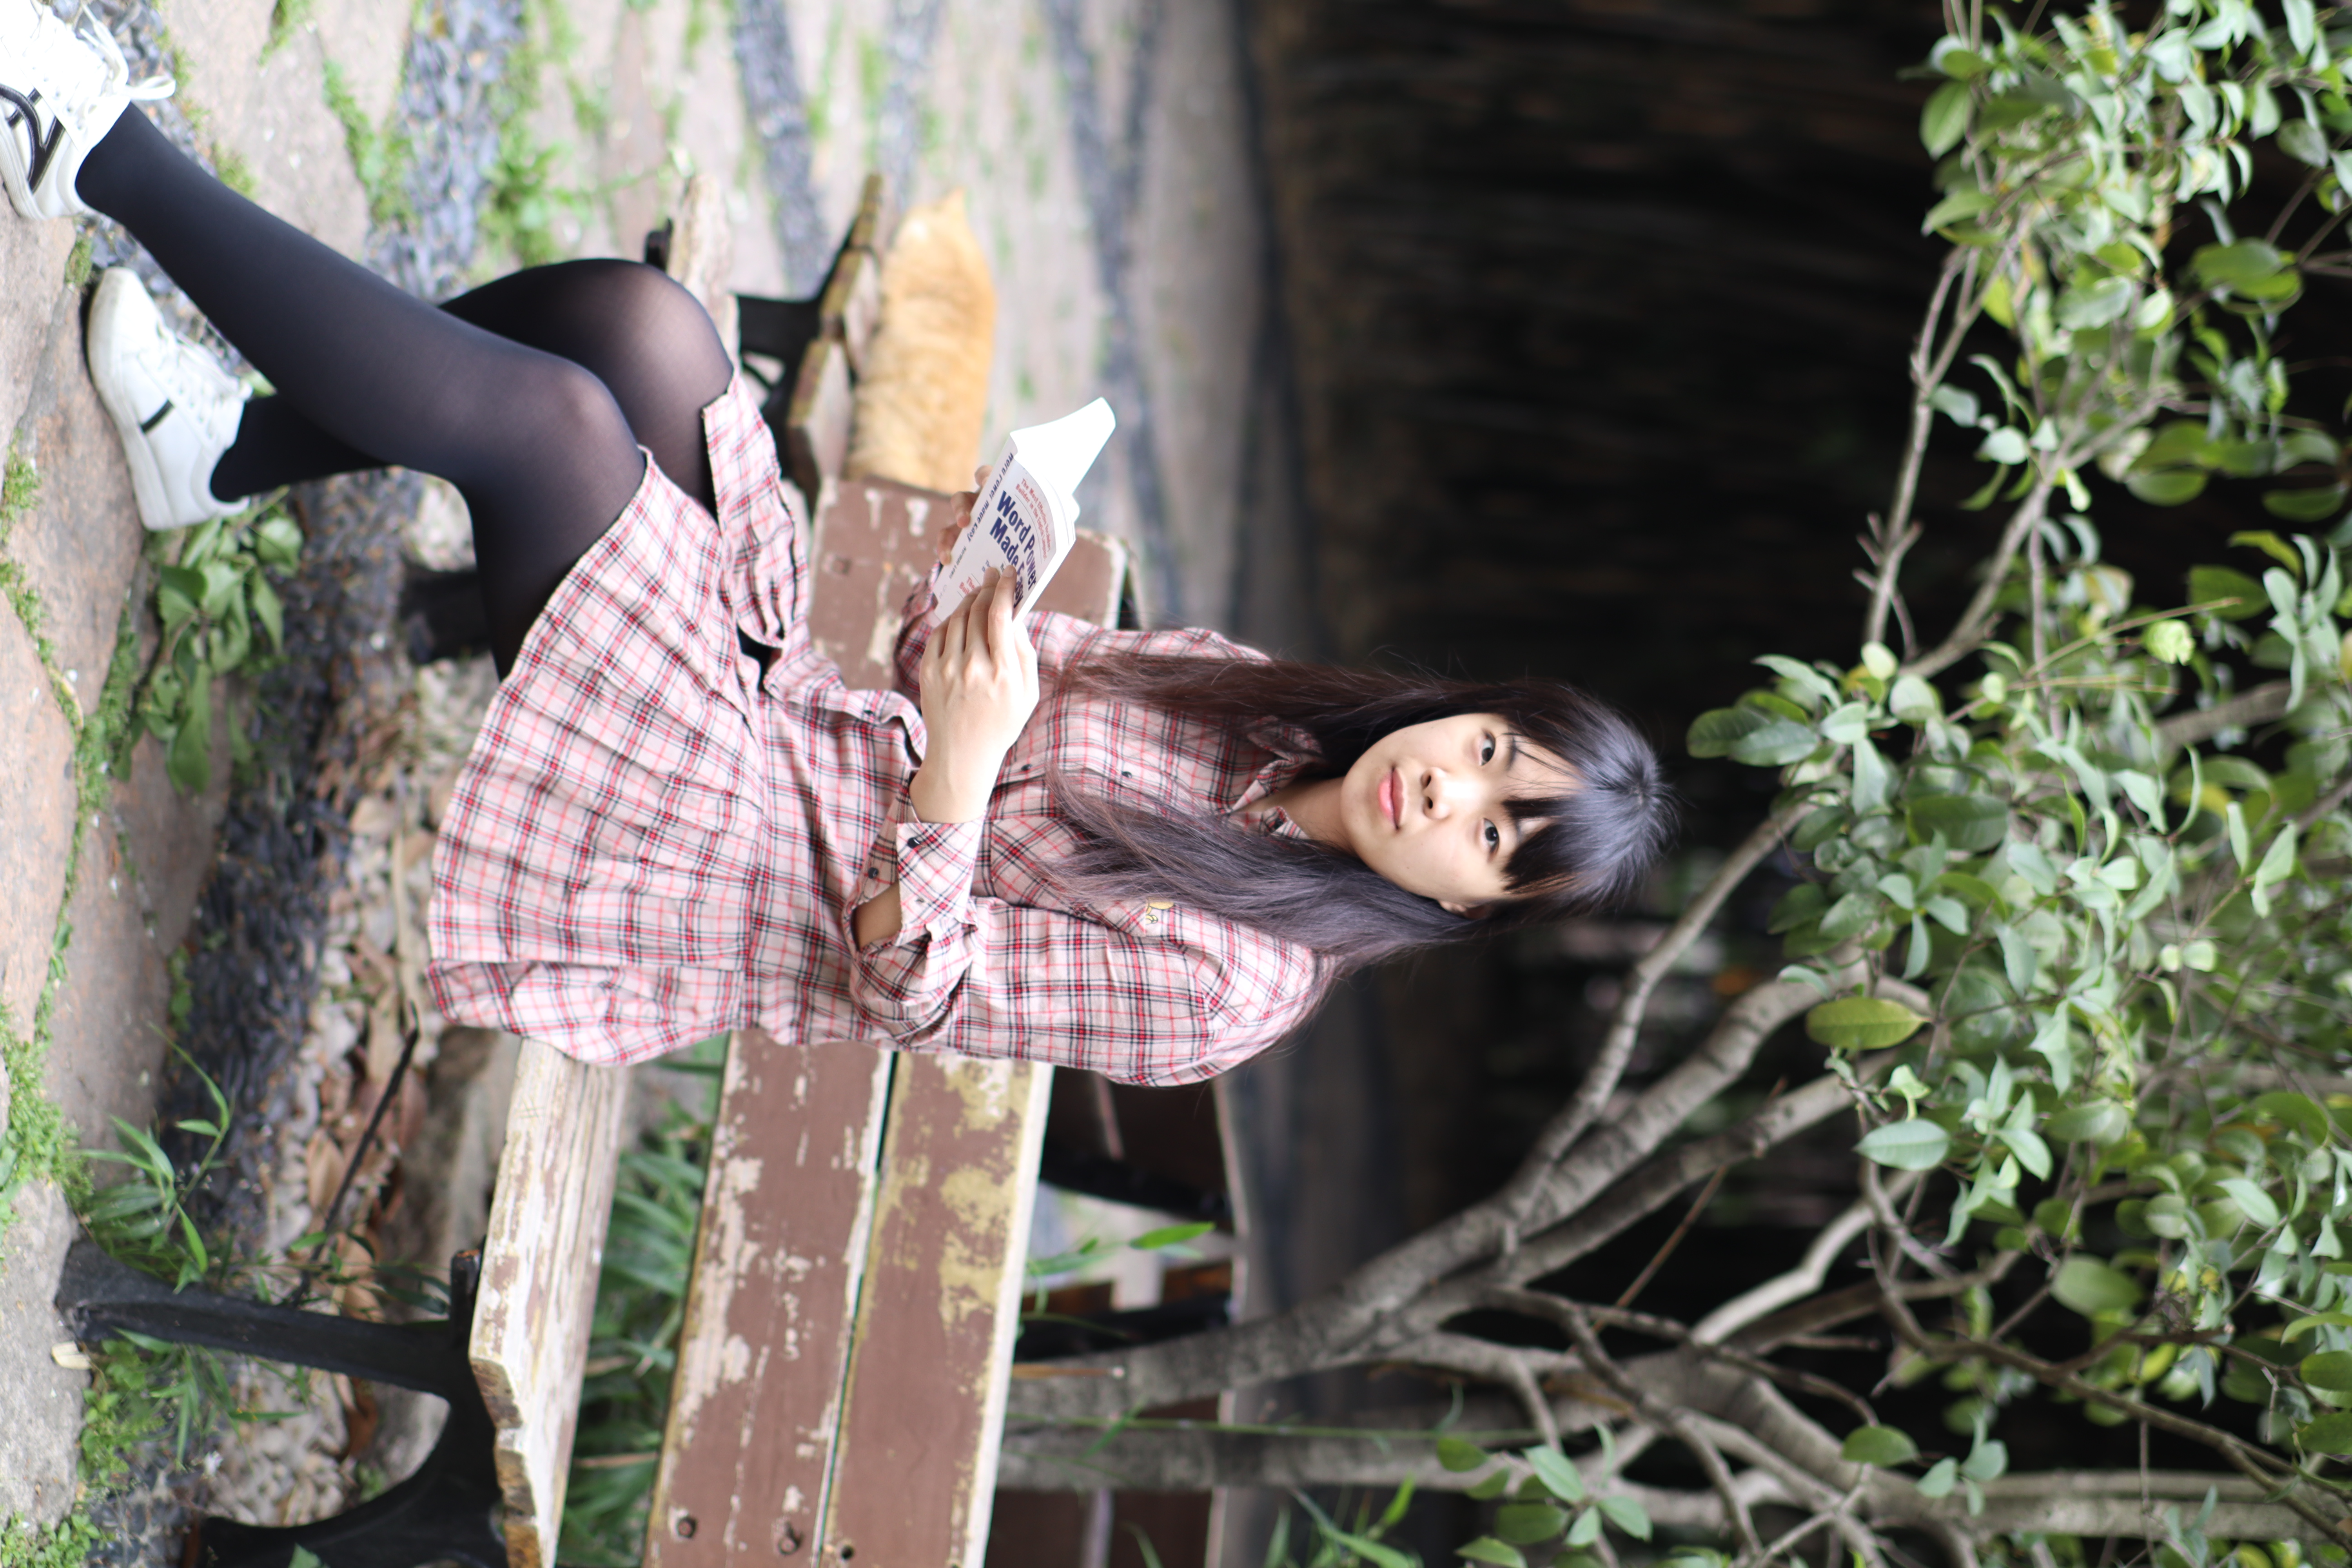
\includegraphics[width=0.9\textwidth,angle=90]{F4}
    \caption{50mm f1.4 1/200}
    \label{F-01}
\end{figure}

上面的照片构图较为传统,主体位于画面中央,竖向拍摄可以几乎将该同学全身放入视野中。
画面中的同学手持一本厚实的书,目光朝向镜头。
该照片由于考虑到大光圈镜头带来的背景虚化,曝光时间较短,但即便如此,
同学手中的书由于光线原因显得过白。

%\bibstyle{unsrt}
%\bibliography{references}{}
\end{document}
